
\documentclass[a4paper,11pt]{article}
\usepackage{csquotes}
\usepackage{marvosym}
\usepackage[a4paper,bottom=1.5in,right=1in,left=1in,top=42mm]{geometry}
\usepackage[fleqn]{mathtools}
\usepackage{graphicx}
\usepackage{hyperref}
\usepackage{colortbl}
\usepackage{underscore}
\usepackage{fancyvrb}
\usepackage{course}
\usepackage{color}
\hypersetup{hidelinks}
\usepackage{fontspec}
\usepackage{mdsymbol}
\settextfont[Scale=1.2]{XB Zar}
%\setlatintextfont[Scale=0.9]{Tahoma}
\lstset{language=C}
\newcommand\tab[1][1cm]{\hspace*{#1}}
\definecolor{sepgray}{gray}{0.8}
\begin{document}


\سربرگ{تمرین پنجم}{\lr{Classification}}{مصطفی قدیمی}
\سؤال{ماشین بردار پشتیبان}

\begin{itemize}
	\item الف)
	\begin{itemize}
		\item یک)
		خیر. اگر 
		$C \rightarrow \infty$
		آن‌گاه برای مجموعه داده‌هایی که به صورت خطی جداپذیر باشند، این اتفاق رخ خواهد داد.
		\footnote{ر.ک. صفحه ۳۳۲ کتاب}
		\item دو)
		همان‌طور که در شکل زیر مشخص است، حالات مختلف ممکن برای $\epsilon$ عبارتند از:
		\begin{itemize}
			\item $\epsilon > 1$: داده به‌طور اشتباه دسته‌بندی شده است.
			\item $\epsilon = 1$:
			یعنی داده روی مرز تصمیم 
			\footnote{\lr{decision boundry}} قرار دارد.
			\item $0 < \epsilon < 1$: داده درست دسته‌بندی شده است اما در \lr{margin} قرار دارد.
			\item $\epsilon = 0$:
			داده درست دسته‌بندی شده است اما ممکن است روی \lr{margin} یا بیرون آن باشد.
		\end{itemize}
		\begin{figure}[hbpt!]
			\centering
			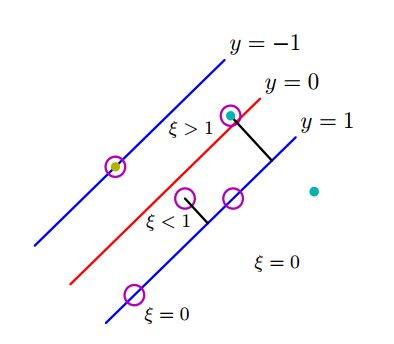
\includegraphics[scale=0.5]{img/1b.jpeg}
			\caption{توصیف معنایی حالات مختلف $\epsilon$}
		\end{figure}
		\item سه)
		حل مسئله با $M$ متغیر به طور کلی پیچیدگی از $O(M^3)$ دارد. در دوگان مسئله‌ی بهینه‌سازی را می‌خواهیم حل کنیم که به‌جای $M$ متغیر، $N$ متغیر دارد. برای تعداد ثابت توابع \lr{basis} چون که 
		$M < N$
		است، استفاده از روش دوگان  به دلیل سرعت کم‌تر خوب نیست. 
		
		استفاده روش دوگان به ما امکان استفاده از هسته‌ها را می‌دهد و می‌توانیم دسته‌بند حاشیه بیشینه 
		\footnote{\lr{maximum margin classifier}}
		را که ابعاد  ویژگی‌های آن بیش‌تر از تعداد نقاط است پیدا کنیم و بسیار کارا است و حتی جواب‌گوی مواقعی که تعداد ویژگی‌ها به بی‌نهایت میل می‌کند می‌باشد.
		\footnote{ر.ک صفجه ۳۲۹ کتاب}
		\item چهار)
		\begin{figure}[hbpt!]
			\centering
			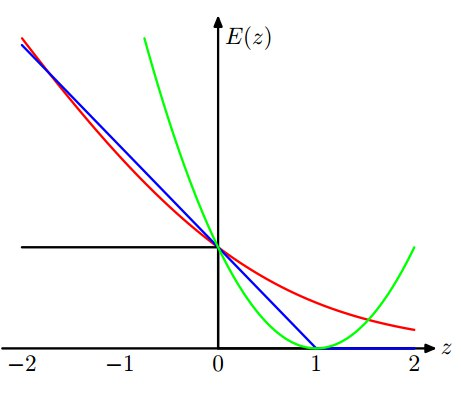
\includegraphics[scale=0.5]{./img/2.jpeg}
			\caption{نمودار آبی: ماشین بردار پشتیبان نرم، نمودار قرمز: 
			\lr{logistic regression}،
			نمودار مشکی: خطای دسته‌بندی
			و نمودار سبر: مربع خطاها
			}
		\end{figure}
		\begin{figure}[hbpt!]
			\centering
			\begin{tikzpicture}
				\begin{axis}[
				xlabel style={below right},
				xlabel=$x$,
				ylabel=$y$,
				ylabel style={above left},
				xmin=-2, xmax=2,
				ymin=0, ymax=2,
				axis lines=center,
				axis on top=true,
				domain=0:1,
				]
				
				\addplot+[color=red,mark=none,samples=200,domain=1:10,smooth,ultra thick] {0} node[below,pos=1,color=black] {};
				
				\addplot+[color=red,mark=none,samples=200,domain=-2:-0,smooth,ultra thick] {2} node[below,pos=1,color=black] {};
				\end{axis}
			\end{tikzpicture}
			\caption{ماشین بردار پشتیبان سخت}
		\end{figure}
	
		\begin{figure}[hbpt!]
			\centering
			\begin{tikzpicture}
			\begin{axis}[
			xlabel style={below right},
			xlabel=$x$,
			ylabel=$y$,
			ylabel style={above left},
			xmin=-2, xmax=2,
			ymin=0, ymax=2,
			axis lines=center,
			axis on top=true,
			domain=0:1,
			]
			
			\addplot+[color=blue,mark=none,samples=200,domain=-2:0,smooth,ultra thick] coordinates{(0, 1)  (-1, 2)}; 
			\addplot+[color=blue,mark=none,samples=200,domain=0:10,smooth,ultra thick] {0} node[below,pos=1,color=black] {};
			
			\end{axis}
			\end{tikzpicture}
			\caption{\lr{perceptron}}
		\end{figure}
	\end{itemize}
	\item ب) 
	در این رابطه حساسیت به داده‌های نویز بیش‌تر می‌شود؛‌ زیرا در مدل  هدف این است که مجموع مجذورات  را کمینه کنیم، بنابراین داده‌های کم‌تری باید به‌طور اشتباه دسته‌بندی شوند و داده‌های نویز اثر و وزن زیادی نسبت به حالت عادی تابع هزینه دارند. 
	\item پ)
	\begin{itemize}
		\item یک)
		$$
		\tilde{L}(a) = \Sigma_{n = 1}^N a_n - \frac{1}{2}\Sigma_{n=1}^N\Sigma_{m=1}^Na_na_mt_nt_mk(x_nm x_m)
		$$
		از آن‌جایی که تعداد داده‌ها ۵ است، بنابراین:
		\footnote{ر.ک. صفحه ۳۲۹ کتاب}
		$$
			\tilde{L}(a) = \Sigma_{n = 1}^5 a_n - \frac{1}{2}\Sigma_{n=1}^5\Sigma_{m=1}^5a_na_mt_nt_mk(x_nm x_m)
		$$
		$$
\tilde{L}(a) = \Sigma_{n = 1}^5 a_n - \frac{1}{2}(a_1^2-4a_1a_4 - 4a_1a_3 - 6a_1a_5 + a_2^2 - 2a_2a_3-4a_2a_4 + 5a_3^2 - 2a_2a_5 + 12a_3a_4 + 14a_3a_5 + 8a_4^2 + 16a_4a_5 + 10a_5^2)
		$$
		$$
		a_n \geq 0 \implies \Sigma_{n = 1}^N a_nt_n = 0 \implies a_1 + a_2 - a_3 - a_4 - a_5 = 0
		$$
		
		\item دو)
		\begin{figure}[hbpt!]
			\centering
			\begin{tikzpicture}
			\begin{axis}[
			axis lines=middle,
			xmin=-1, xmax=4,
			ymin=-1, ymax=4,
			xtick=\empty, ytick=\empty
			]
			\addplot [only marks] table {
				0 1
				1  0

			};
			\addplot [only marks, mark=o] table {
				1  2
				2  2
				1  3

			};
			\addplot [domain=-10:10, samples=2, dashed] {-1*x+2};
			\end{axis}
			\end{tikzpicture}
		\end{figure}
				چون نقطه‌‌های ۴ و ۵ نمی‌توانند بردار پشتیبان باشند، داریم:
	$$
	a_4 = a_5 = 0 \implies a_1 + a_2 - a_3   = 0 \implies a_1 + a_2 = a_3
	$$
		\item سه)
		با جای‌گذاری نتیجه‌ی بالا در معادله‌ی قسمت «۱» داریم:
		$$
		\tilde{L}(a) = a_1 + a_2 + a_3 - \frac{1}{2}(a_1^2 + a_2^2 + 5a_3^2 - 4a_1a_3 - 2a_2a_3)
		$$
		
		\item چهار) 
		برای حل مسئله‌ی بهینه‌سازی باید لاگرانژ تابع را برابر با صفر قرار دهیم.
		$$
		\nabla \tilde{L}(a) = 0 \implies \begin{cases}
		 1 - \frac{1}{2}(2a_1 - 4a_3) = 0 & with \: respect \: to \: a_{1} \\
 		 1 - \frac{1}{2}(2a_2 - 2a_3) = 0 & with \: respect \: to \: a_{2} \\
 		 1 - \frac{1}{2}(-4a_1 - 2a_2 + 10a_3) = 0 & with \: respect \: to \: a_{3}
		\end{cases}
		$$
		از قسمت قبلی دریافتیم که $a_1 + a_2 = a_3$. حال با حذف $a_3$ از دو معادله داریم:
		$$
		a_1 - a_2 = a_3
		$$
		
		با جای‌گذاری این نتایج در معادلات بالا، به دست‌ می‌آوریم:
		$$
		a_1 = a_3 = \frac{1}{3}, \: a_2 = 0
		$$
		
		\item پنج)
		
		$$
		y(x) = wx + b \implies w = \frac{1}{3}(x_1 - x_3) = (-\frac{1}{3}, -\frac{1}{3}), \: b = \frac{2}{3} \implies y(x) = (-\frac{1}{3}, -\frac{1}{3})x + \frac{2}{3}
		$$
	\end{itemize}
\end{itemize}

\newpage
\سؤال{مشتق‌گیری}

هر کدام از روابط زیر را ثابت کنید.
\begin{itemize}
	\item 
	$\frac{\partial a^tx}{\partial x} = a$
	
	$$
	\frac{\partial a^tx}{\partial x} = 
	\frac{\partial \begin{pmatrix}
		a_1 & \dots & a_n \\
		\end{pmatrix}
		\begin{pmatrix}
		x_1 \\
		\vdots \\
		x_n \\
		\end{pmatrix}}{\partial x}
	= \frac{\partial (a_1x_1 + \dots + a_nx_n)}{\partial x}
	$$
	اگر $f = (a_1x_1 + \dots + a_nx_n)$ داریم:
	$$
	\frac{\partial a^tx}{\partial x} = 	\frac{\partial f}{\partial x} = 
	\begin{pmatrix}
		\frac{\partial f}{\partial x_1} \\
		 \dots \\ \frac{\partial f}{\partial x_n}\\
	\end{pmatrix} =
	\begin{pmatrix}
	a_1 \\
	\dots \\
	 a_n \\
	\end{pmatrix}
	= a
	$$
	\item 
	$\frac{\partial x^tAx}{\partial x} = 2xA$
\end{itemize}
\newpage
\سؤال{درخت تصمیم}

\newpage
\سؤال{یادگیری جمعی}

\begin{itemize}
	\item الف)
	نامساوی \lr{Jensen}:
	
	$$
	f(\Sigma_{i = 1}^M\lambda_i x_i) \leq \Sigma_{i = 1}^M\lambda_if(x_i)
	$$
	همان‌طور که در صورت سوال گفته شده است برای $E_{avg}$ داریم:
	$$
	E_{avg} = \frac{1}{M} \Sigma_{i = 1}^{M}E_x[(h_m(x) - h(x)^2]
	$$
	حال اگر $\frac{1}{M}$ را به درون سیگما ببریم، داریم:
	$$
	E_{avg} = E_x[\Sigma_{m=1}^M  \frac{1}{M}(h_m(x) - h(x))^2]
	$$
	
	حال با توجه به نامساوی \lr{Jensen} و محدب بودن تابع داریم:
	$$
	(\Sigma_{m=1}^M\frac{1}{M}(h_m(x) - h(x))^2 \leq \Sigma_{m=1}^M\frac{1}{M}(h_m(x) - h(x))^2
	$$
	$$
	\implies E_{com} \leq E_{avg}
	$$
	\item ب)
	
	$$
	E_{avg} = \frac{1}{M} \Sigma_{m=1}^M E_x[(h_m(x) - h(x))^2]
	$$
	
	$$
	E_{com} = E_x[(\frac{1}{M} \Sigma_{m=1}^M h_m(x) - h(x))^2] = E_x[(\frac{1}{M} \Sigma_{m=1}^M h_m(x) - h(x)) (\frac{1}{M} \Sigma_{l=1}^M h_l(x) - h(x))]
	$$
	حال اگر یکی از عامل‌های $\frac{1}{M}$ را به دلیل ثابت بودن از داخل امید ریاضی بیرون بیاوریم، به دلیل فرضیات یعنی
	 $$
	 \forall m \neq l \: E[(h_m(x) - h(x))(h_l(x)-h(x))] = 0
	 $$
	 داریم:
	 $$
	 E_{com} = \frac{1}{M}(\frac{1}{M} \Sigma_{m=1}^M E_x[(h_m(x) - h(x))^2]) = \frac{1}{M}E_{avg}
	 $$
\end{itemize}

\newpage
\سؤال{}


اگر $y_n = y(x_n, w)$ آن‌گاه داریم:
$$
y^{noisy}_n = w_0 + \Sigma_i^{D} w_i(x_{ni} + \epsilon_{ni}) 
= y_n + \Sigma_i^{D}w_i\epsilon_{ni}
$$

حال با استفاده از 
$
E_D(w) = \frac{1}{2} \Sigma_{n = 1}^{N}(y(x_n, w) - t_n)^2
$
داریم:
$$
E^{noisy} = 
\frac{1}{2}\Sigma_{n = 1}^{N}(y^{noisy}_{n} - t_n)^2 
= \frac{1}{2}\Sigma_{n =  1}^{N}(y_n^{noisy \: 2} - 2y_n^{noisy}t_n + t_n^2)
$$

$$
\rightarrow E^{noisy} = 
\frac{1}{2} \Sigma_{n = 1}^{N}(y_n^2 + 2y_n\Sigma_{i = 1}^{D}w_i\epsilon_{ni} + (\Sigma_{i = 1}^{D}w_i\epsilon_{ni})^2 - 2t_ny_n - 2t_n\Sigma_{i = 1}^{D}w_i\epsilon_{ni} + t_n^2)
$$

حال اگر امید ریاضی $E^{noisy}$را بگیریم که جملع‌ی  $2y_n\Sigma_{i = 1}^{D}w_i\epsilon_{ni}$ و جمله‌ی 
$
- 2t_n\Sigma_{i = 1}^{D}w_i\epsilon_{ni} + t_n^2
$
به دلیل 
$
\mathbb{E}(\epsilon_{ni}) = 0
$
حذف می‌شوند. 
\\
به دلیل استقلال $\epsilon_{ni}$ها داریم:
$$
\mathbb{E}[(\Sigma_{i = 1}^{D}w_i\epsilon_{ni})^2] = \Sigma_{i = 1}^{D}w_i^2\sigma^2
$$

$$
\rightarrow \mathbb{E}[E^{noisy}] = E_D + \frac{1}{2} \Sigma_{i = 1}^{D} w_i^2\sigma^2
$$
\newpage
\سؤال{}

به دلیل افزایش ویژگی‌ها کارایی در مدل $D_2$  کاهش م‌یابد. اما به دلیل یکسان بودن (هم‌بسنگی ۱) تغییری در دقت آن به وجود نمی‌آید.
\newpage
\سؤال{گاوسی چندمتغیره}

\begin{enumerate}
	\item 

	اگر 
	$
	a = \begin{pmatrix}
	3 & -2 & 1 \\
	\end{pmatrix}^T
	$
	آن‌گاه داریم: 
	
	$$a^TX=3X_1 -2X_2 + X_2
	\rightarrow a^TX \sim N(a^T\mu, \: a^T\Sigma a)
	$$
	$$a^T\mu = 
	\begin{pmatrix}
	3 & -2 & 1 \\
	\end{pmatrix}
	\begin{pmatrix}
	2 \\
	-3 \\
	1
	\end{pmatrix}
	= 13
	$$
	
	$$a^T\Sigma a = 
	\begin{pmatrix}
	3 & -2 & 1 
	\end{pmatrix}
	\begin{pmatrix}
	1 & 1 & 1 \\
	1 & 3 & 2 \\
	1 & 2 & 2 \\
	\end{pmatrix}
	\begin{pmatrix}
	3 \\
	-2 \\
	1
	\end{pmatrix}
	= 9
	$$
	
	در نتیجه‌ توزیع آن برابر با $N_3(13, \: 9)$ است.
	\item 
	اگر 
	$a = \begin{pmatrix}
	a_1 & a_2 \\
	\end{pmatrix}^T$ آن‌گاه داریم:
	
	$$Y = X_2 - a^T\begin{pmatrix}
	X_1 \\
	X_3\\
	\end{pmatrix}
	= -a_1X_1 + X_2 - a_2X_3
	$$
	حال اگر 
	$A = \begin{pmatrix}
	0 & 1 & 0 \\
	-a_1 & 1 & -a_2\\
	\end{pmatrix}$
	آن‌گاه داریم: 
	$$AX = \begin{pmatrix}
	X_2\\
	Y
	\end{pmatrix}
	\sim N(A\mu, \: A\Sigma A^T)
	$$
	که 
	$$
	A\Sigma A^T = \begin{pmatrix}
	0 & 1 & 0 \\
	-a_1 & 1 & -a_2
	\end{pmatrix}
	\begin{pmatrix}
	1 & 1 & 1 \\
	1 & 3 & 2 \\
	1 & 2 & 2 \\
	\end{pmatrix}
	\begin{pmatrix}
	0 & -a_1 \\
	1 & 1 \\
	0 & -a_2\\
	\end{pmatrix}
	$$
	$$
	= \begin{pmatrix}
	3 & -a_1 - 2a_2 + 3 \\
	-a_1 - 2a_2 + 3 & a_1^2 - 2a_1 - 4a_2 + 2a_1a_2 + 2a_2^2 + 3\\
	\end{pmatrix}
	$$.
	چون می‌خواهیم $X_2$ و $Y$ مستقل باشند، باید $-a_1 - 2a_2 + 3 = 0$. بنابراین،
	برای $v \in \mathbb{R}$ داریم:
	$$a = \begin{pmatrix}
	3 \\
	0
	\end{pmatrix}
	+ v \begin{pmatrix}
	-2 \\
	1
	\end{pmatrix}
	$$
	
\end{enumerate}
\newpage
\سؤال{\lr{ML \& MAP}}

\begin{enumerate}
	\item پیدا کردن \lr{joint}
	$$f_{\mu, \: X, \: Y}(t, x, y) = f(x, y | t) f(t)$$
	فرمول توزیع نرمال به صورت زیر است:
	$$N(x, \mu, \sigma^2) = \frac{1}{\sqrt{2\pi} \sigma^2} e^{\frac{-(x - \mu) ^2}{2\sigma^2}}$$
	حال با توجه به این‌که واریانس برابر با ۱ است، داریم:
	$$f_{\mu, \: X, \: Y}(t, x, y) = f(x, y | t) f(t) = \begin{cases}
	\frac{1}{2\pi} e^{-\frac{(x - t)^2 + (y - t)^2}{2}} & t \in [0, 1] \\
	0 & otherwise \\
	\end{cases}$$
	\item 
	پیدا کردن \lr{posterior}
	$$MAP = arg max f(t|x, y) = \frac{f(x, y | t) f(t)}{f(x, y)} \sim arg max \log{f(t | x, y) \times 1}$$ 
	با مشتق‌گیری از رابطه‌ی بالا و قرار دادن آن برابر با صفر به رابطه‌ی $t = \frac{x + y}{2}$ می‌رسیم.
	\item 
	ارزیابی:
	\begin{itemize}
		\item آ)
	$$x = \frac{3}{4}, y = 1 \rightarrow t = \frac{\frac{7}{4}}{2} = \frac{7}{8}$$
		\item ب)
		$$x = \frac{1}{2}, y = 2 \rightarrow \frac{\frac{5}{2}}{2} = \frac{5}{4} > 1$$
		از آن‌جایی که تابع لگاریتم یک تابع یک‌به‌یک و صعودی است و مقدار احتمال بیش‌تر از یک نداریم، باید این احتمال را ۱ در نظر بگیریم.
	\end{itemize}
\end{enumerate}
\newpage
\end{document}
